\documentclass[a4paper]{article}
\addtolength{\hoffset}{-2.25cm}
\addtolength{\textwidth}{4.5cm}
\addtolength{\voffset}{-3.25cm}
\addtolength{\textheight}{5cm}
\setlength{\parindent}{15pt}

\usepackage[unicode=true, colorlinks=false, hidelinks]{hyperref}
\usepackage[utf8]{inputenc}
\usepackage[english, russian]{babel}
\usepackage{mathtext}
\usepackage[T2A, TS1]{fontenc}
\usepackage{microtype} % Slightly tweak font spacing for aesthetics
\usepackage{amsthm, amssymb, amsmath, amsfonts, nccmath}
\usepackage{nicefrac}
\usepackage{epstopdf}
\usepackage[export]{adjustbox}
\usepackage{float} % Improved interface for floating objects
\usepackage{graphicx, multicol} % Enhanced support for graphics
\usepackage{pdfrender,xcolor}
\usepackage{breqn}
\usepackage{mathtools}
\usepackage{titling}
\usepackage{bm}
\usepackage{centernot}
\usepackage[cal=boondoxo,calscaled=.96]{mathalpha}
\usepackage{marvosym, wasysym} % More symbols
\usepackage{rotating} % Rotation tools
\usepackage{censor} % Facilities for controlling restricted text
\usepackage{indentfirst}
\usepackage{svg}

\DeclareMathOperator{\rad}{rad}
\DeclareMathOperator{\imid}{mid}
\DeclareMathOperator{\sign}{sign}
\newcommand{\mbb}[1]{\mathbb{#1}}
\newcommand{\mbf}[1]{\mathbf{#1}}

\usepackage{array}
\newcolumntype{C}[1]{>{\centering\let\newline\\\arraybackslash\hspace{0pt}}m{#1}}

\usepackage{fancyhdr}
\pagestyle{fancy}
\fancyhead{}\renewcommand{\headrulewidth}{0pt}
\fancyfoot[L]{}
\fancyhead{}
\fancyfoot{}
\fancyfoot[R]{\thepage}
\begin{document}
\large
\begin{center}
    Санкт-Петербургский политехнический университет\\
    Высшая школа прикладной математики и\\вычислительной физики,\\ 
    Физико-механический институт\\
    \vspace{3em}
    Направление подготовки\\
    01.03.02 «Прикладная математика и информатика»\\
    \vspace{10em}
    \Large
    Отчет по лабораторной работе №2 \\
    по дисциплине «Интервальный анализ»
    \vspace{19em}
    \large
\end{center}
Выполнил студент гр. 5030102/80201\\
Кирпиченко С. Р.\\
Руководитель\\
Баженов А. Н.
\vspace{10em}
\begin{center}
    Санкт-Петербург\\
    2021
\end{center}
\thispagestyle{empty}
\newpage
\tableofcontents
\addtocontents{toc}{~\hfill\textbf{Страница}\par}
\newpage
\listoffigures
\addtocontents{lof}{~\hfill\textbf{Страница}\par}
\newpage
\section{Постановка задачи}
\subsection{Внешнее оценивание множества решений ИСЛАУ в $\mathbb{IR}$ }
Дана ИСЛАУ 
\begin{equation}\label{lin}
    \begin{cases}
    \mbf{x}_1+2\mbf{x}_2=[2,\:4]\\
    \mbf{x}_1 - [1,\:2]\cdot\mbf{x}_2=0
    \end{cases}
\end{equation}

Необходимо произвести оценку внешнего множества решений с помощью метода Кравчика и:
\begin{itemize}
    \item Определить спектральный радиус матрицы
    \item Провести оценку начального бруса решения
    \item Проиллюстрировать положение брусов при итерациях
    \item Проиллюстрировать радиусы брусов при итерациях
    \item Проиллюстрировать расстояние центров брусов при итерациях до центра последнего бруса
\end{itemize}


\subsection{Внешнее оценивание множества решений нелинейных задач в $\mathbb{IR}$ }
Дана нелинейная система уравнений 
\begin{equation}\label{nelin}
    \begin{cases}
    \mbf{x}_1+2\mbf{x}_2=[2,\:4]\\
    \frac{\mbf{x}_1}{\mbf{x}_2} = [1,\:2]
    \end{cases}
\end{equation}

Необходимо произвести оценку внешнего множества решений с помощью метода Кравчика и:
\begin{itemize}
    \item Проиллюстрировать положение брусов при итерациях
    \item Проиллюстрировать радиусы брусов при итерациях
    \item Проиллюстрировать расстояние центров брусов при итерациях до центра последнего бруса
\end{itemize}
\section{Теория}
\subsection{Внешнее множество решений}
Под внешним множеством решений понимается объединенное множество решений, образованное решениями всех точечных систем $F(a,x)=b$
$$\Xi_{\mathrm{uni}}=\{x\in\mbb{R}^n|\exists a\in\mbf{a},\:\exists b\in\mbf{b}:\:F(a,x)=b\}$$
\subsection{Метод Кравчика}
Метод Кравчика - это итерационная процедура уточнения двусторонней границы решений системы n уравнений с n неизвестными $F(\mbf{x})=0,\:\mbf{x}\in\mbf{X}\subset\mbb{IR}^n$, определенной на некотором брусе $\mbf{X}$. Данный метод позволяет не только произвести оценку, но и убедиться, что решений не существует.

Отображение $\mathcal{K}(\mbf{X}, \overline{x})=\overline{x}-\Lambda\cdot F(\overline{x})-(I -\Lambda\cdot \mbf{L})\cdot(\mbf{X}-\overline{x})$ называется оператором Кравчика на $\mbf{X}$ относительно точки $\overline{x}$. Если $\rho(I -\Lambda\cdot \mbf{L})<1$, то по теореме Шрёдера у отображения существует единственная неподвижная точка, являющаяся решением рассматриваемой системы уравнений.

Метод Кравчика заключается в построении последовательности $\{\mbf{X}^k\}_{k=0}^\infty$ по формуле 
$$\mbf{X}^{k+1}=\mbf{X}^{k}\cap\mathcal{K}(\mbf{X}^k, \overline{x}^k)$$ Начальный брус, точки $\overline{x}$, предобуславливатель $\Lambda$ и матрица $\mbf{L}$ выбираются исходя из эмпирических соображений для каждой конкретной системы уравнений. Для решения задачи (\ref{nelin}) будут использованы следующие формулы:
$$\mbf{X}^0=\begin{pmatrix}[0.1,\: 5]\\ [0.1,\: 5]\end{pmatrix},\;\overline{x}^k=\mathrm{mid}\:\mbf{X}^k,\;\Lambda=\Lambda(\mbf{x})=(\mathrm{mid}\:J(\mbf{x}))^{-1},\;\mbf{L}=\mbf{L}(\mbf{x})=J(\mbf{x})$$
где $J(\mbf{x})$ - якобиан.

Частный случай метода Кравчика для ИСЛАУ выглядит следующим образом:
$$\mbf{x}^{k+1}=\left(\Lambda\cdot\mbf{b}+(I-\Lambda\cdot\mbf{A})\cdot\mbf{x}^k\right)\cap\mbf{x}^{k},$$
где $\mbf{A}$ - матрица ИСЛАУ, $\mbf{b}$ - вектор правой части. Для решения задачи (\ref{lin}) предобуславливатель будет выбран как $\Lambda=(\mathrm{mid}\:\mbf{A})^{-1}$. 
\subsection{Выбор начального приближения}
Для систем общего вида выбор начального бруса - отдельная задача, которая не поддается обобщению. Тем не менее, в случае ИСЛАУ справедливо следующее утверждение:
$$\eta=||I-\Lambda\cdot\mbf{A}||_\infty<1\Rightarrow\Xi_{\mathrm{uni}}\subset\begin{pmatrix}[-\theta,\:\theta]\\ \cdots\\ [-\theta,\:\theta]\end{pmatrix},\;\theta=\frac{||\Lambda\cdot\mbf{b}||_\infty}{1-\eta}$$

В качестве начального приближения при решении задачи (\ref{lin}) будет использована эта оценка внешнего множества решений.
\section{Реализация}
Для осуществления вычислений и визуализации результатов использовалась среда Matlab с библиотекой интервальной арифметики IntLab.
\section{Результаты}
\subsection{Спектральный радиус $|I-\Lambda\mbf{A}|$}
Для того, чтобы итерационный процесс сходился, необходимо, чтобы спектральный радиус матрицы $|I-\Lambda\mbf{A}|$ был меньше 1.
$$|I-\Lambda\mbf{A}|\approx\begin{pmatrix}0&0.2857\\ 0&0.1429\end{pmatrix}$$
$$\rho(|I-\Lambda\mbf{A}|)\approx0.1429<1$$

Итерационный процесс сходящийся, можно пользоваться методом Кравчика.
\subsection{Оценка бруса начального положения}
$||I-\Lambda\cdot\mbf{A}||_\infty\approx0.2857<1$. Следовательно, можно воспользоваться описанным выше способом выбора $\mbf{X}^0$.
$$\theta=\frac{||\Lambda\cdot\mbf{b}||_\infty}{1-\eta}\approx2.4\Rightarrow\mbf{X}^0=\begin{pmatrix}[-2.4,\: 2.4]\\ [-2.4,\: 2.4]\end{pmatrix}$$
\subsection{Результаты применения метода Кравчика для задачи (\ref{lin})}
Если построить 4 прямые и найти область, образованную их пересечением, то получим $\Xi_{\mathrm{uni}}$ для рассматриваемой задачи.
\begin{figure}[H]
    \centering
    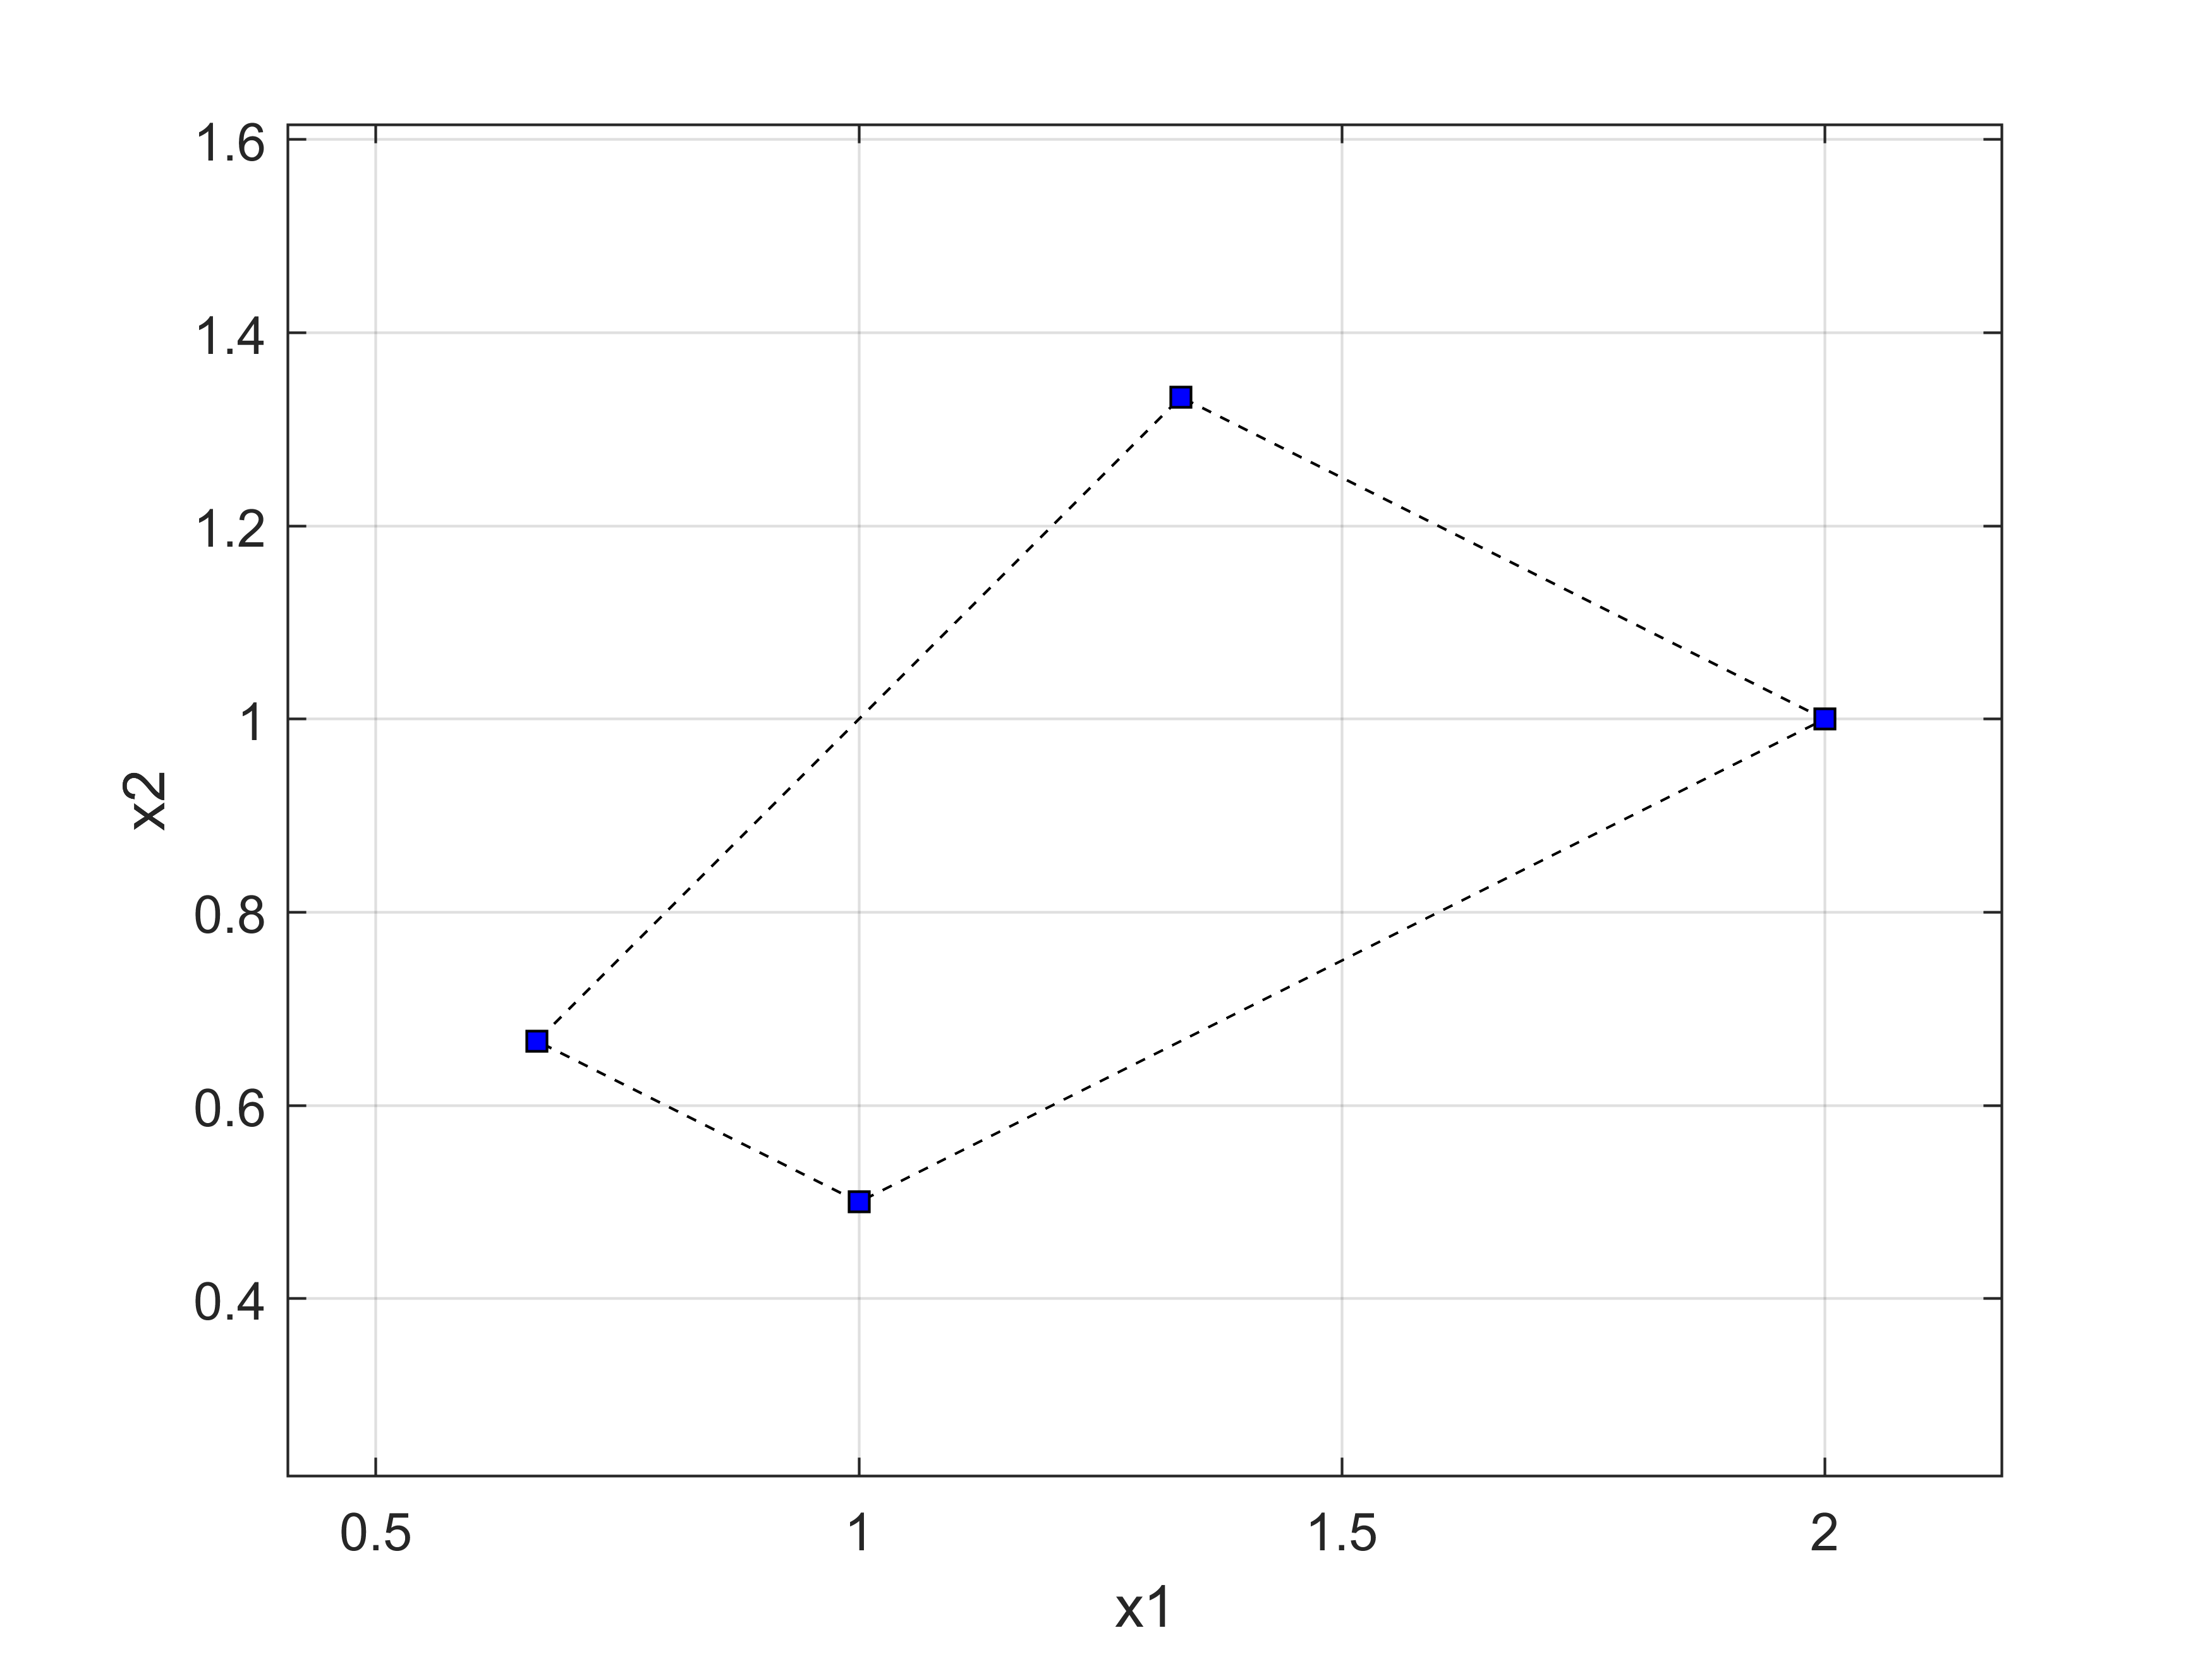
\includegraphics[width=15cm]{img/xi_uni.png}
    \caption{Множество $\Xi_{\mathrm{uni}}$}
    \label{fig:xi}
\end{figure}
Результатом выполнения метода Кравчика являются следующие брусы:
\begin{figure}[H]
    \centering
    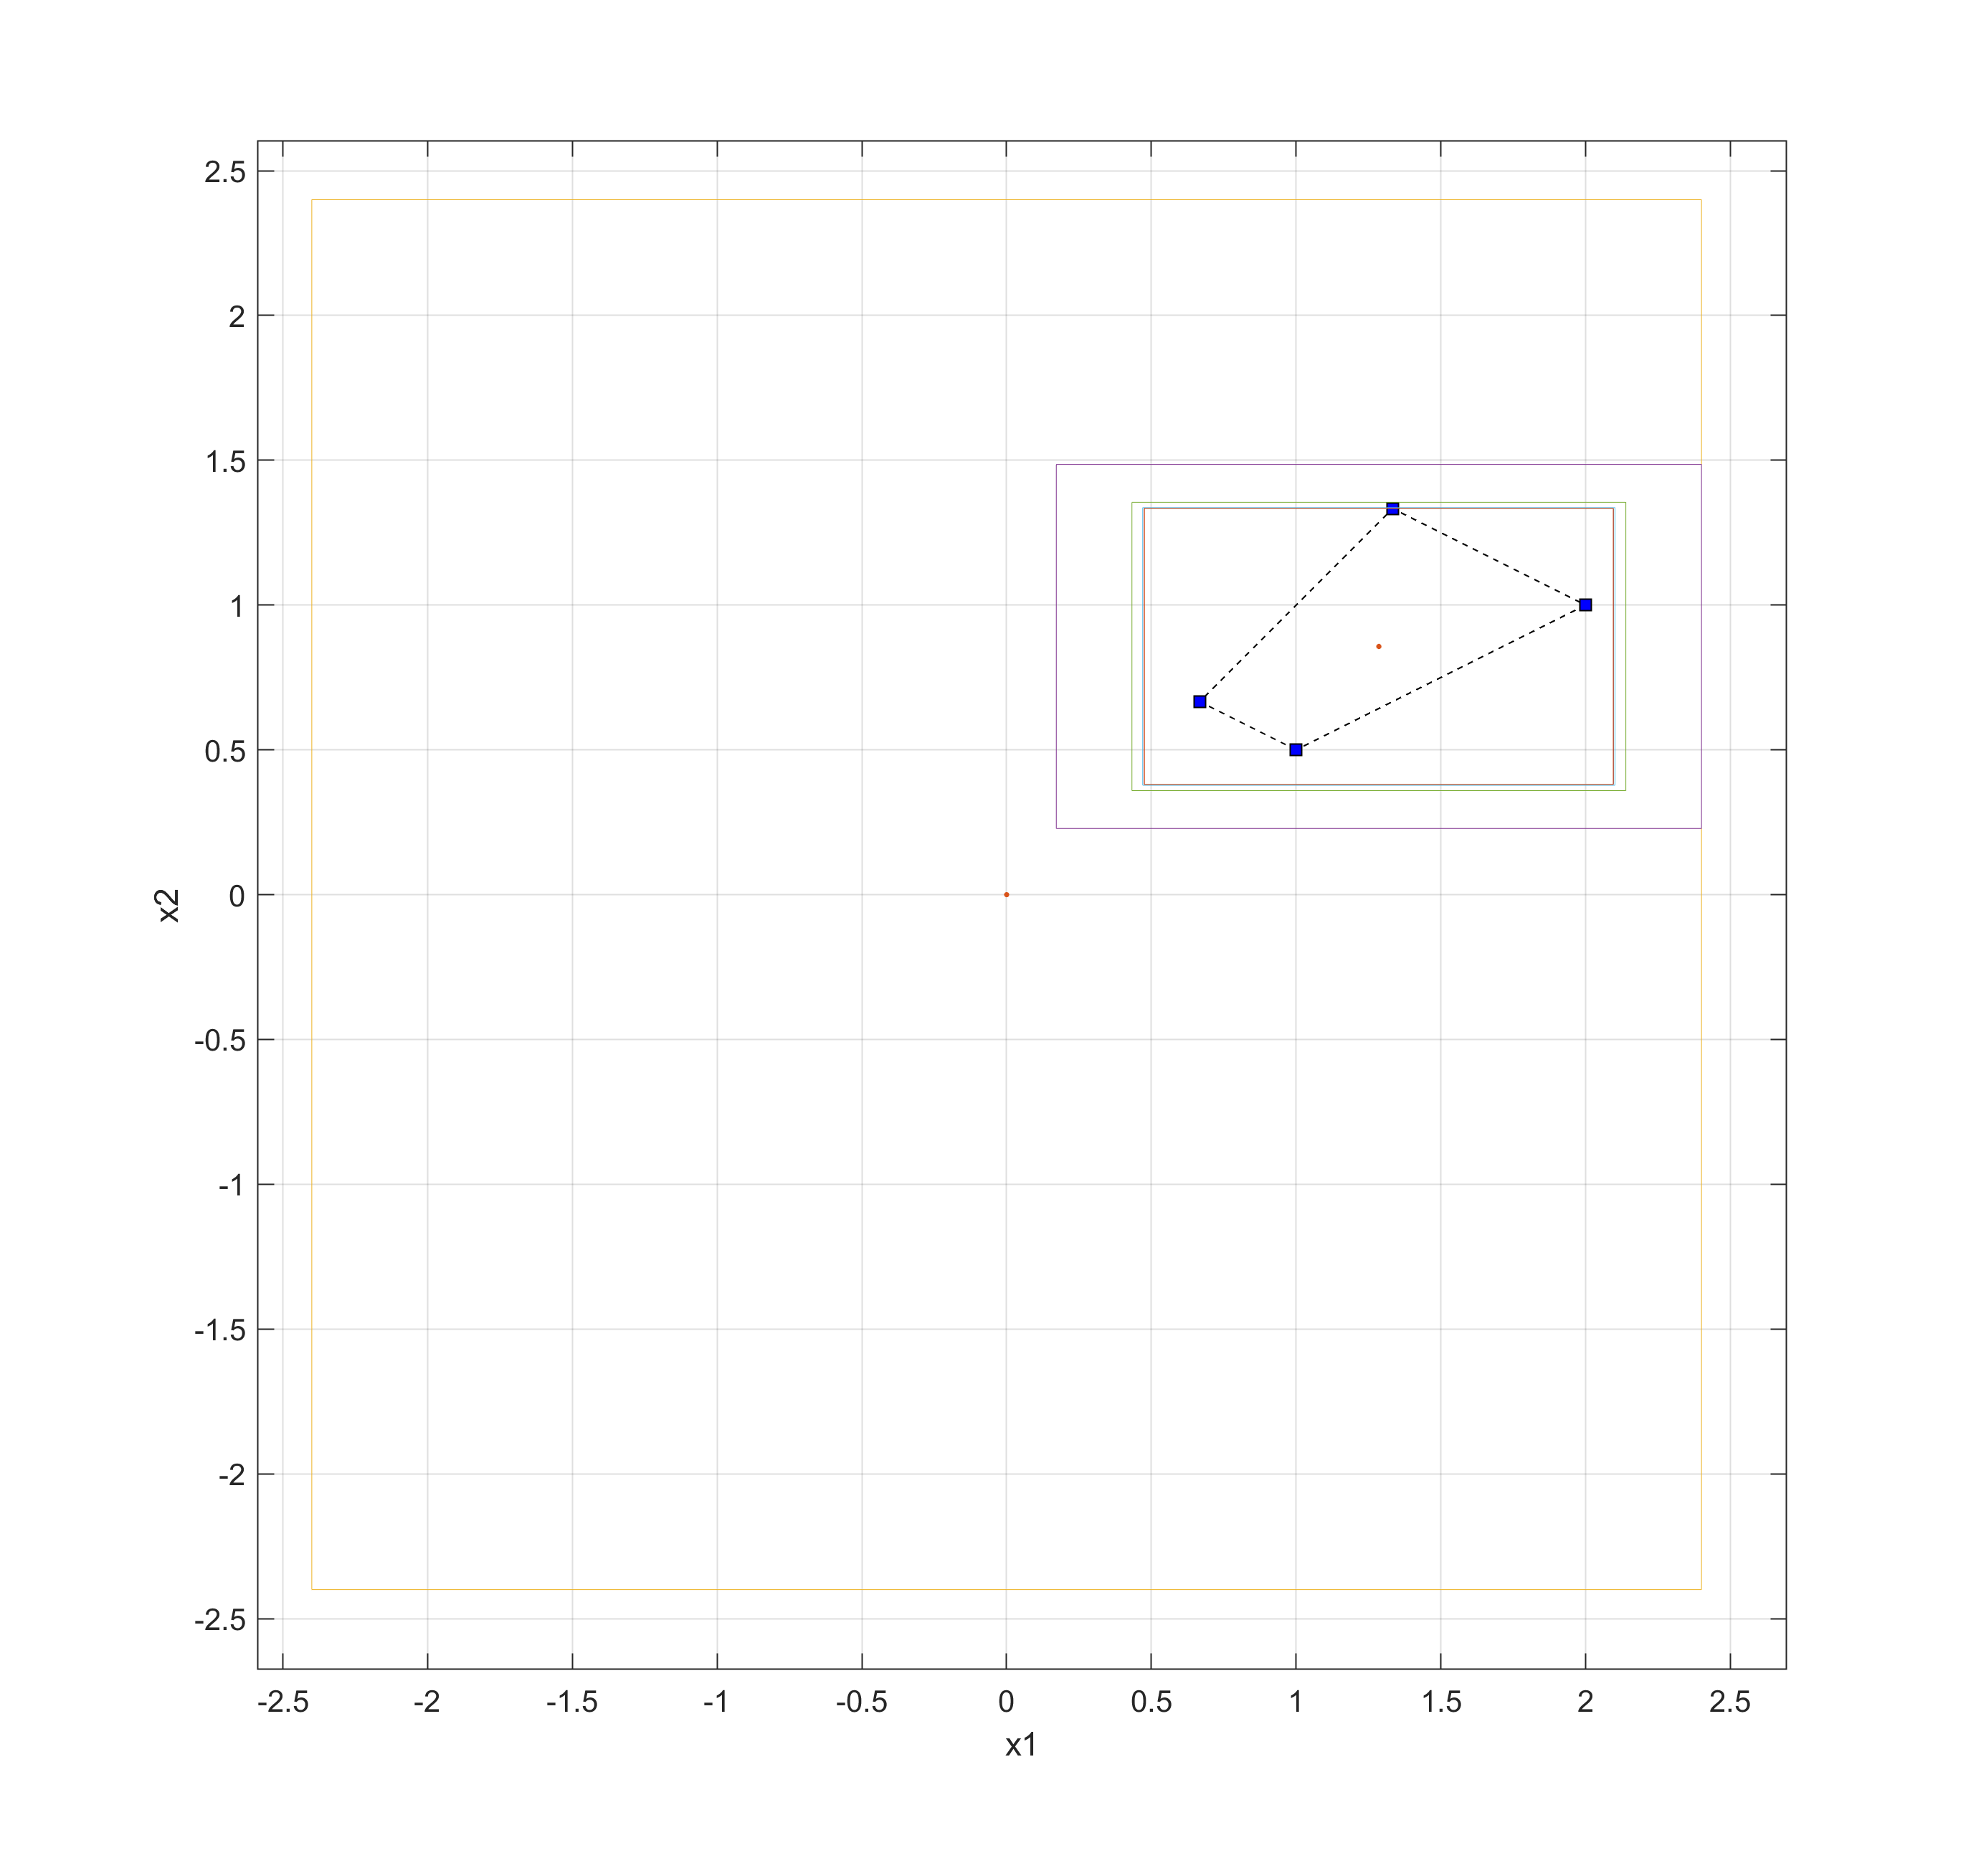
\includegraphics[width=8cm]{img/lin_mar.png}
    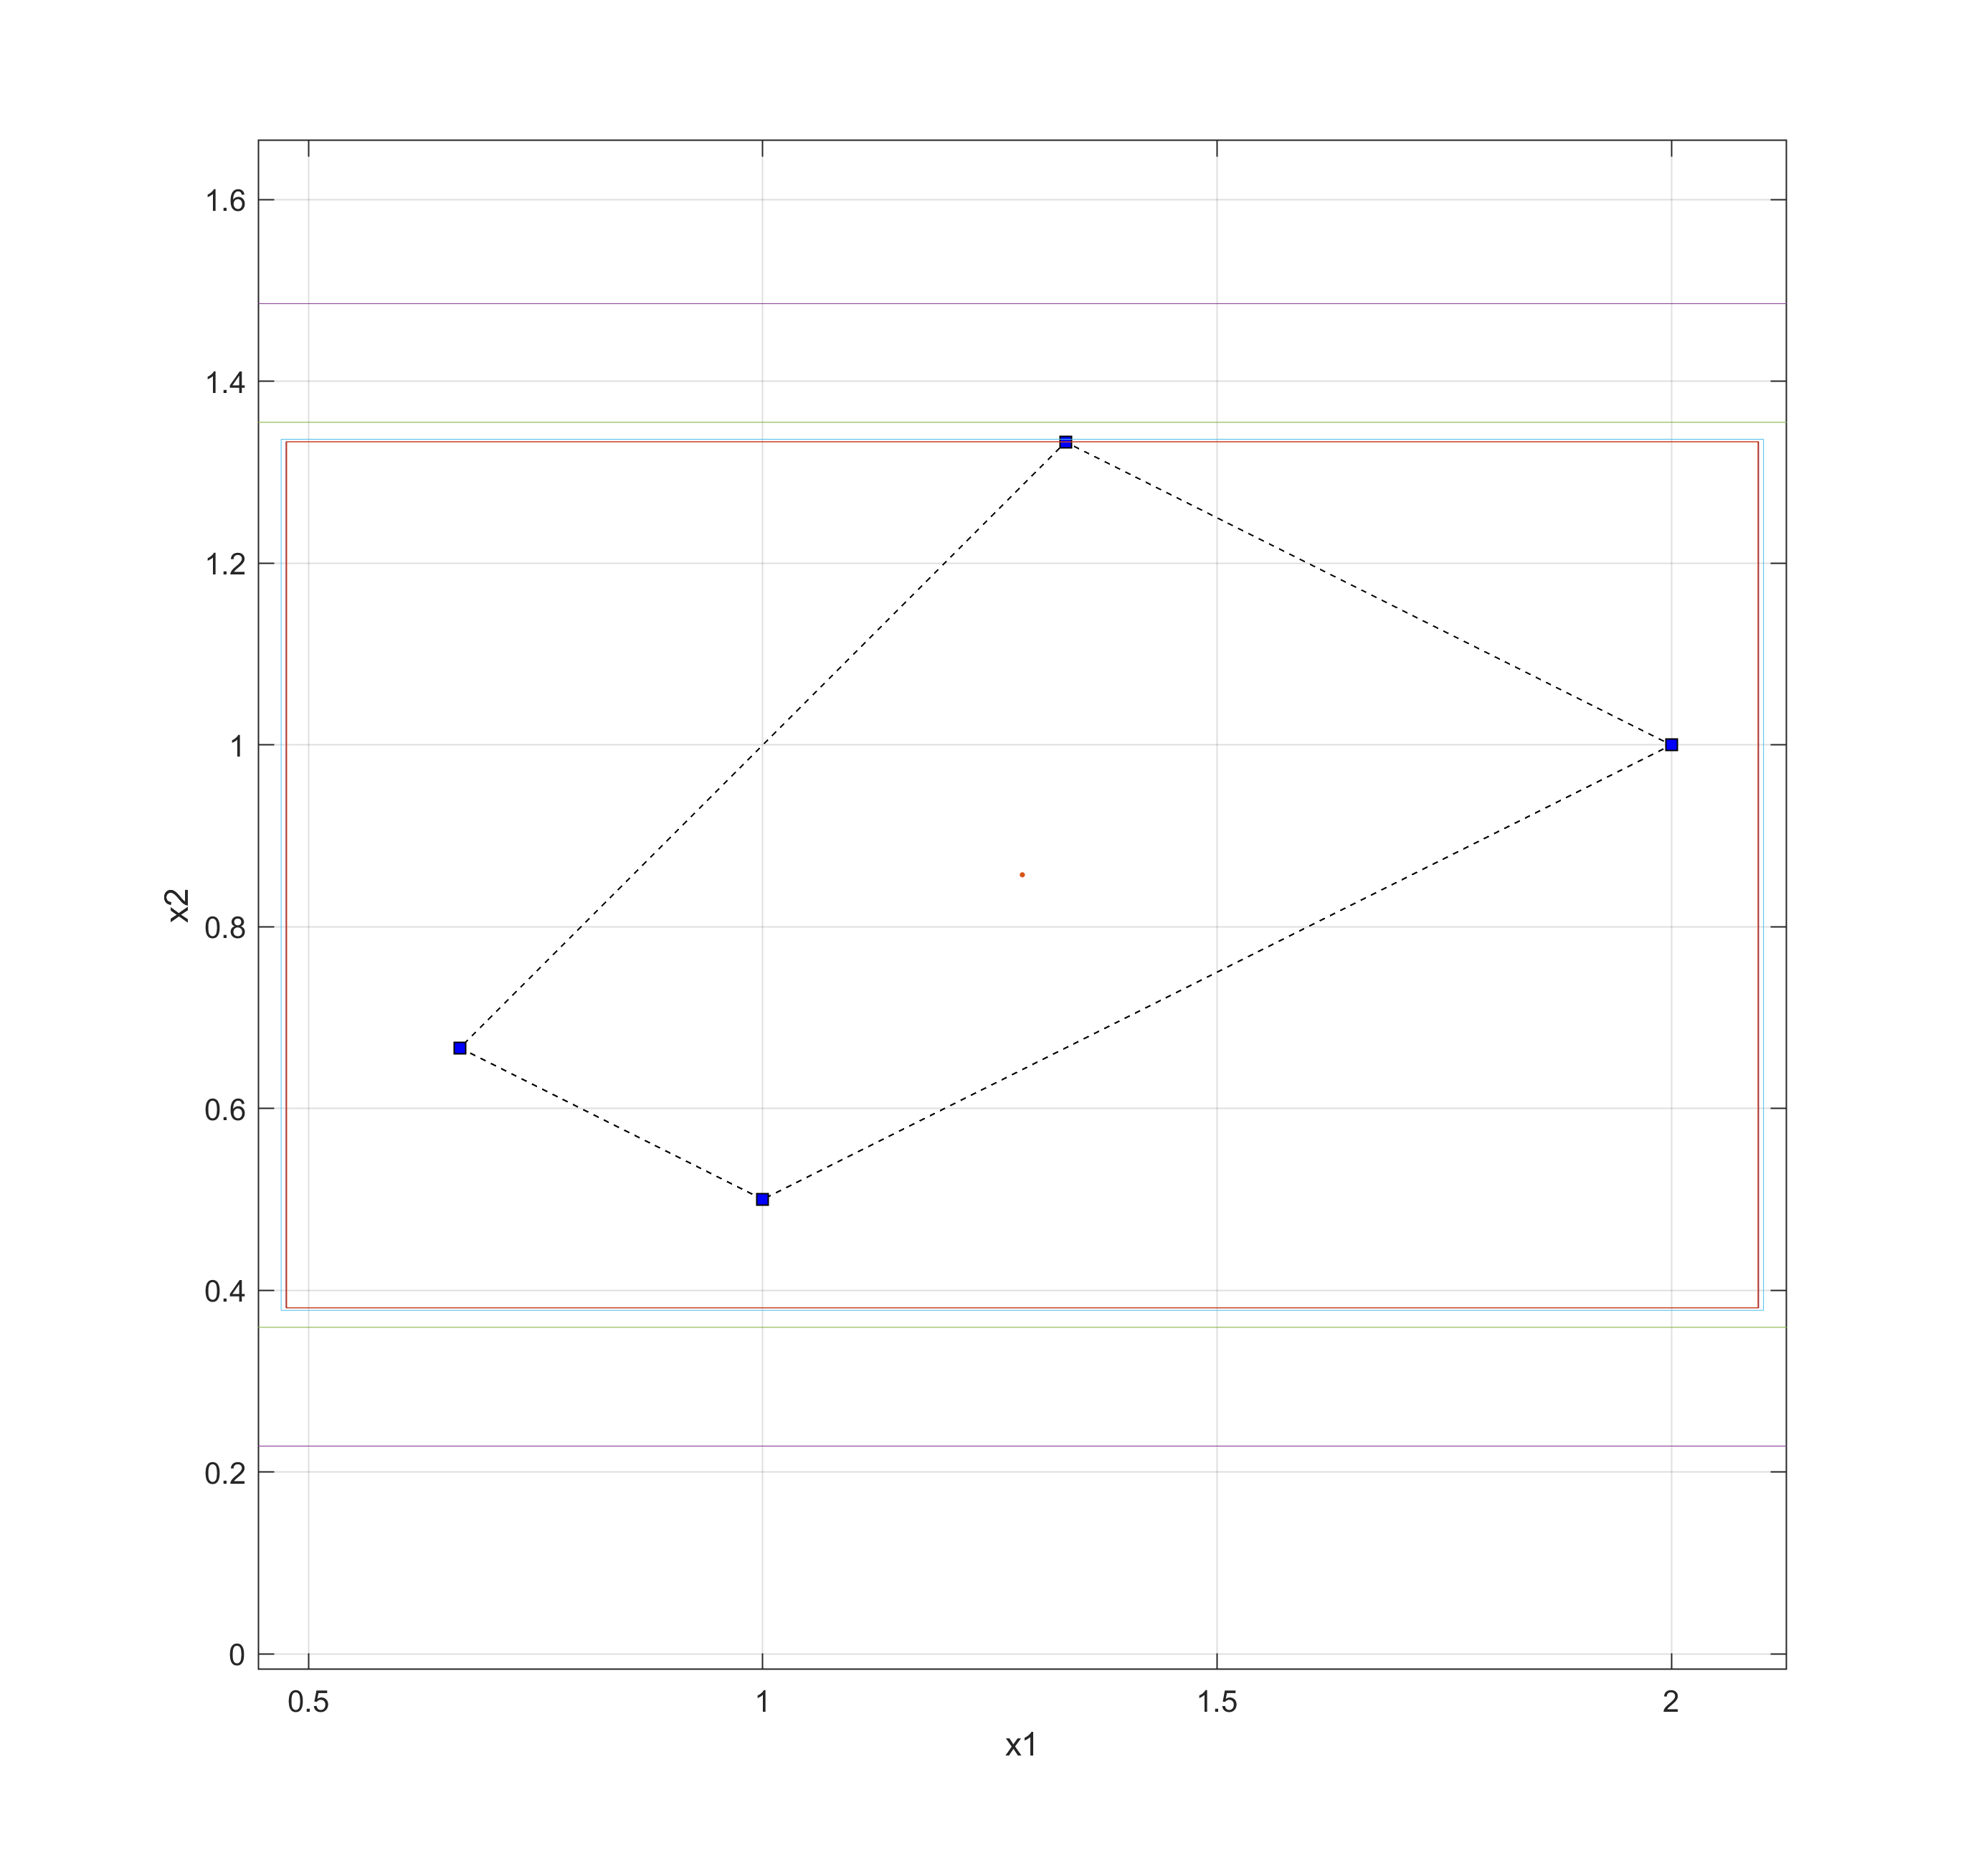
\includegraphics[width=8cm]{img/lin_mar_close.png}
    \caption{Иллюстрация работы метода Кравчика для ИСЛАУ}
    \label{fig:islau_krav}
\end{figure}
\begin{figure}[H]
    \centering
    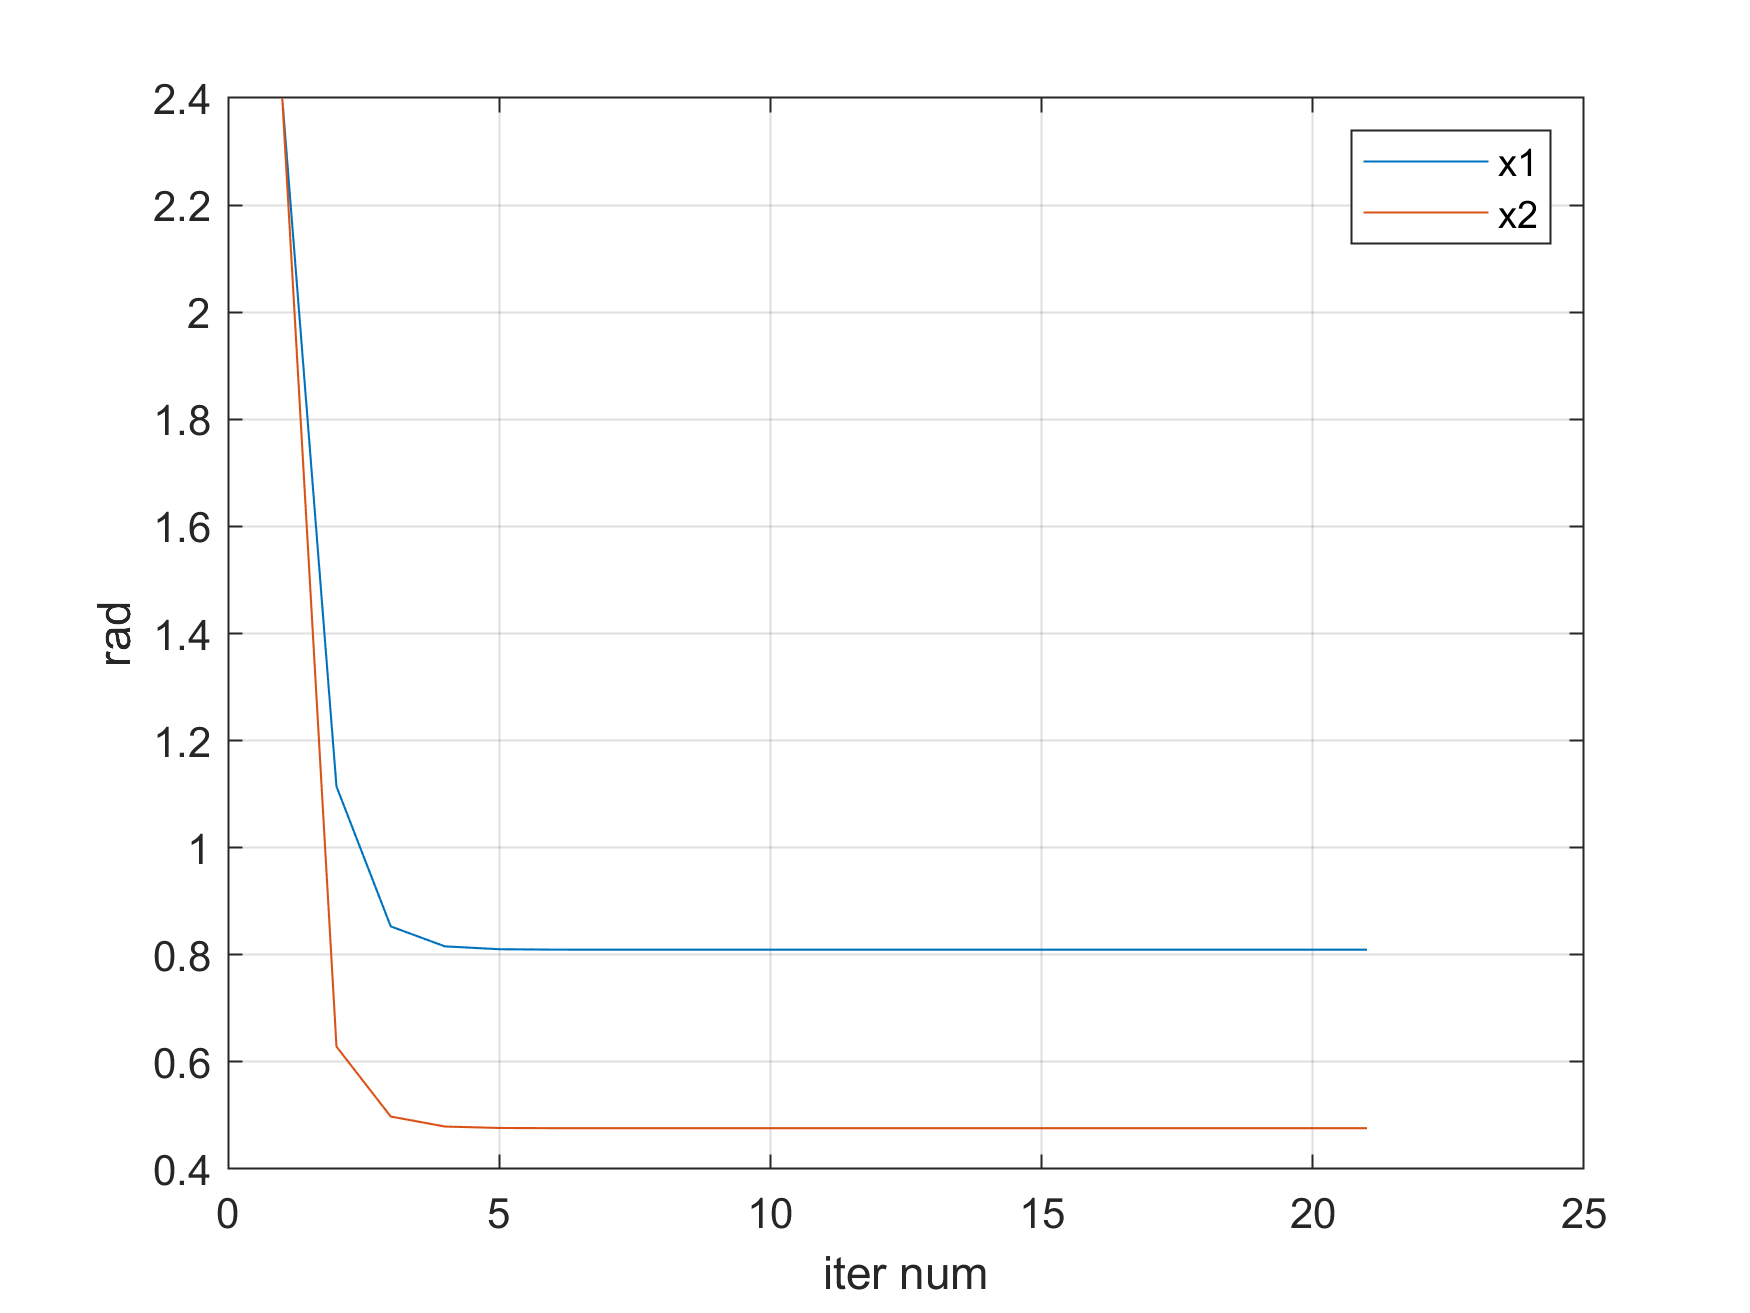
\includegraphics[width=15cm]{img/lin_rad.png}
    \caption{График радиусов брусов для ИСЛАУ}
    \label{fig:islau_rad}
\end{figure}
\begin{figure}[H]
    \centering
    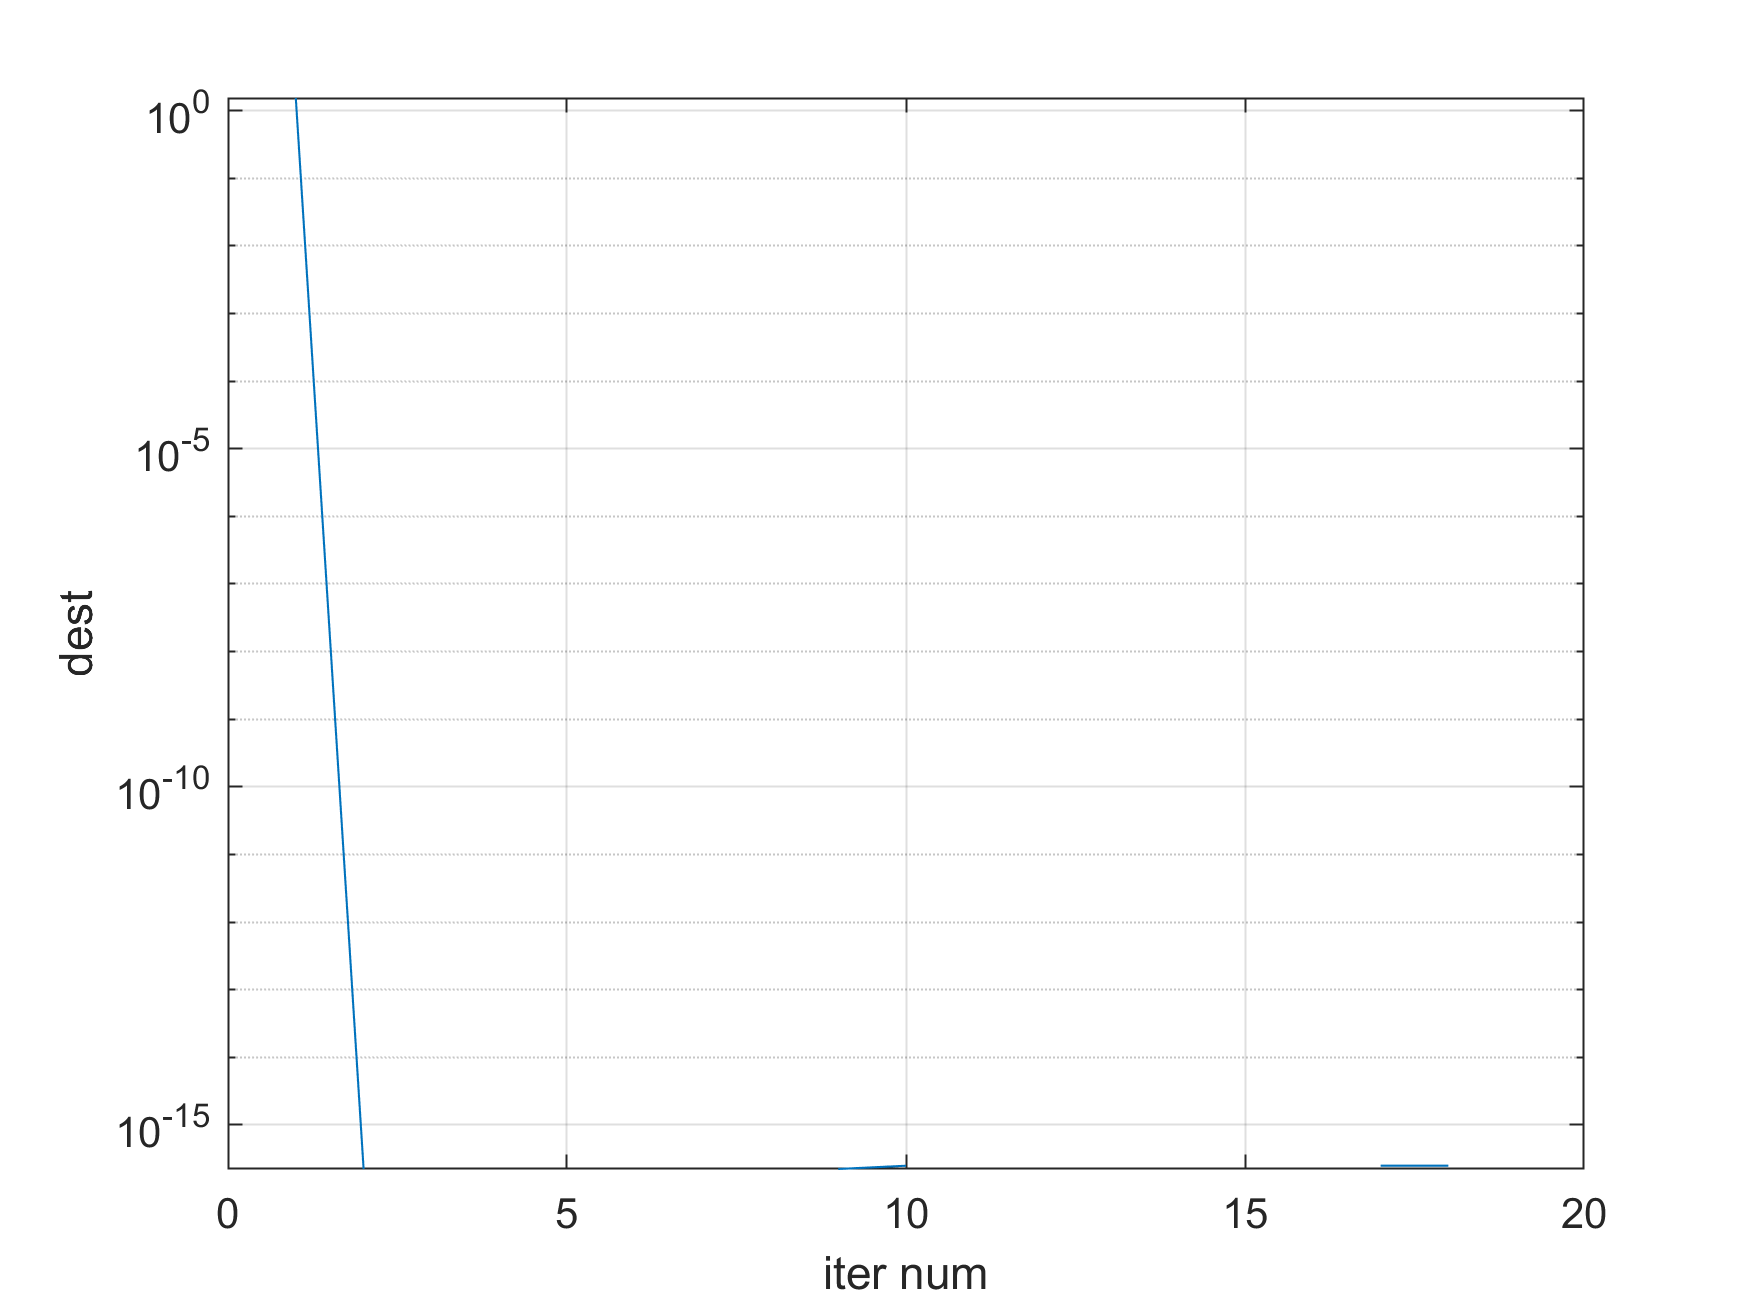
\includegraphics[width=15cm]{img/lin_dest.png}
    \caption{График сходимости брусов для ИСЛАУ}
    \label{fig:islau_dest}
\end{figure}
\subsection{Результаты применения метода Кравчика для задачи (\ref{nelin})}
Так как задачи являются эквивалентными в смысле геометрической интерпретации, то $\Xi_{\mathrm{uni}}$ остается таким же, как на графике \ref{fig:xi}.

Результатом выполнения метода Кравчика являются следующие брусы:
\begin{figure}[H]
    \centering
    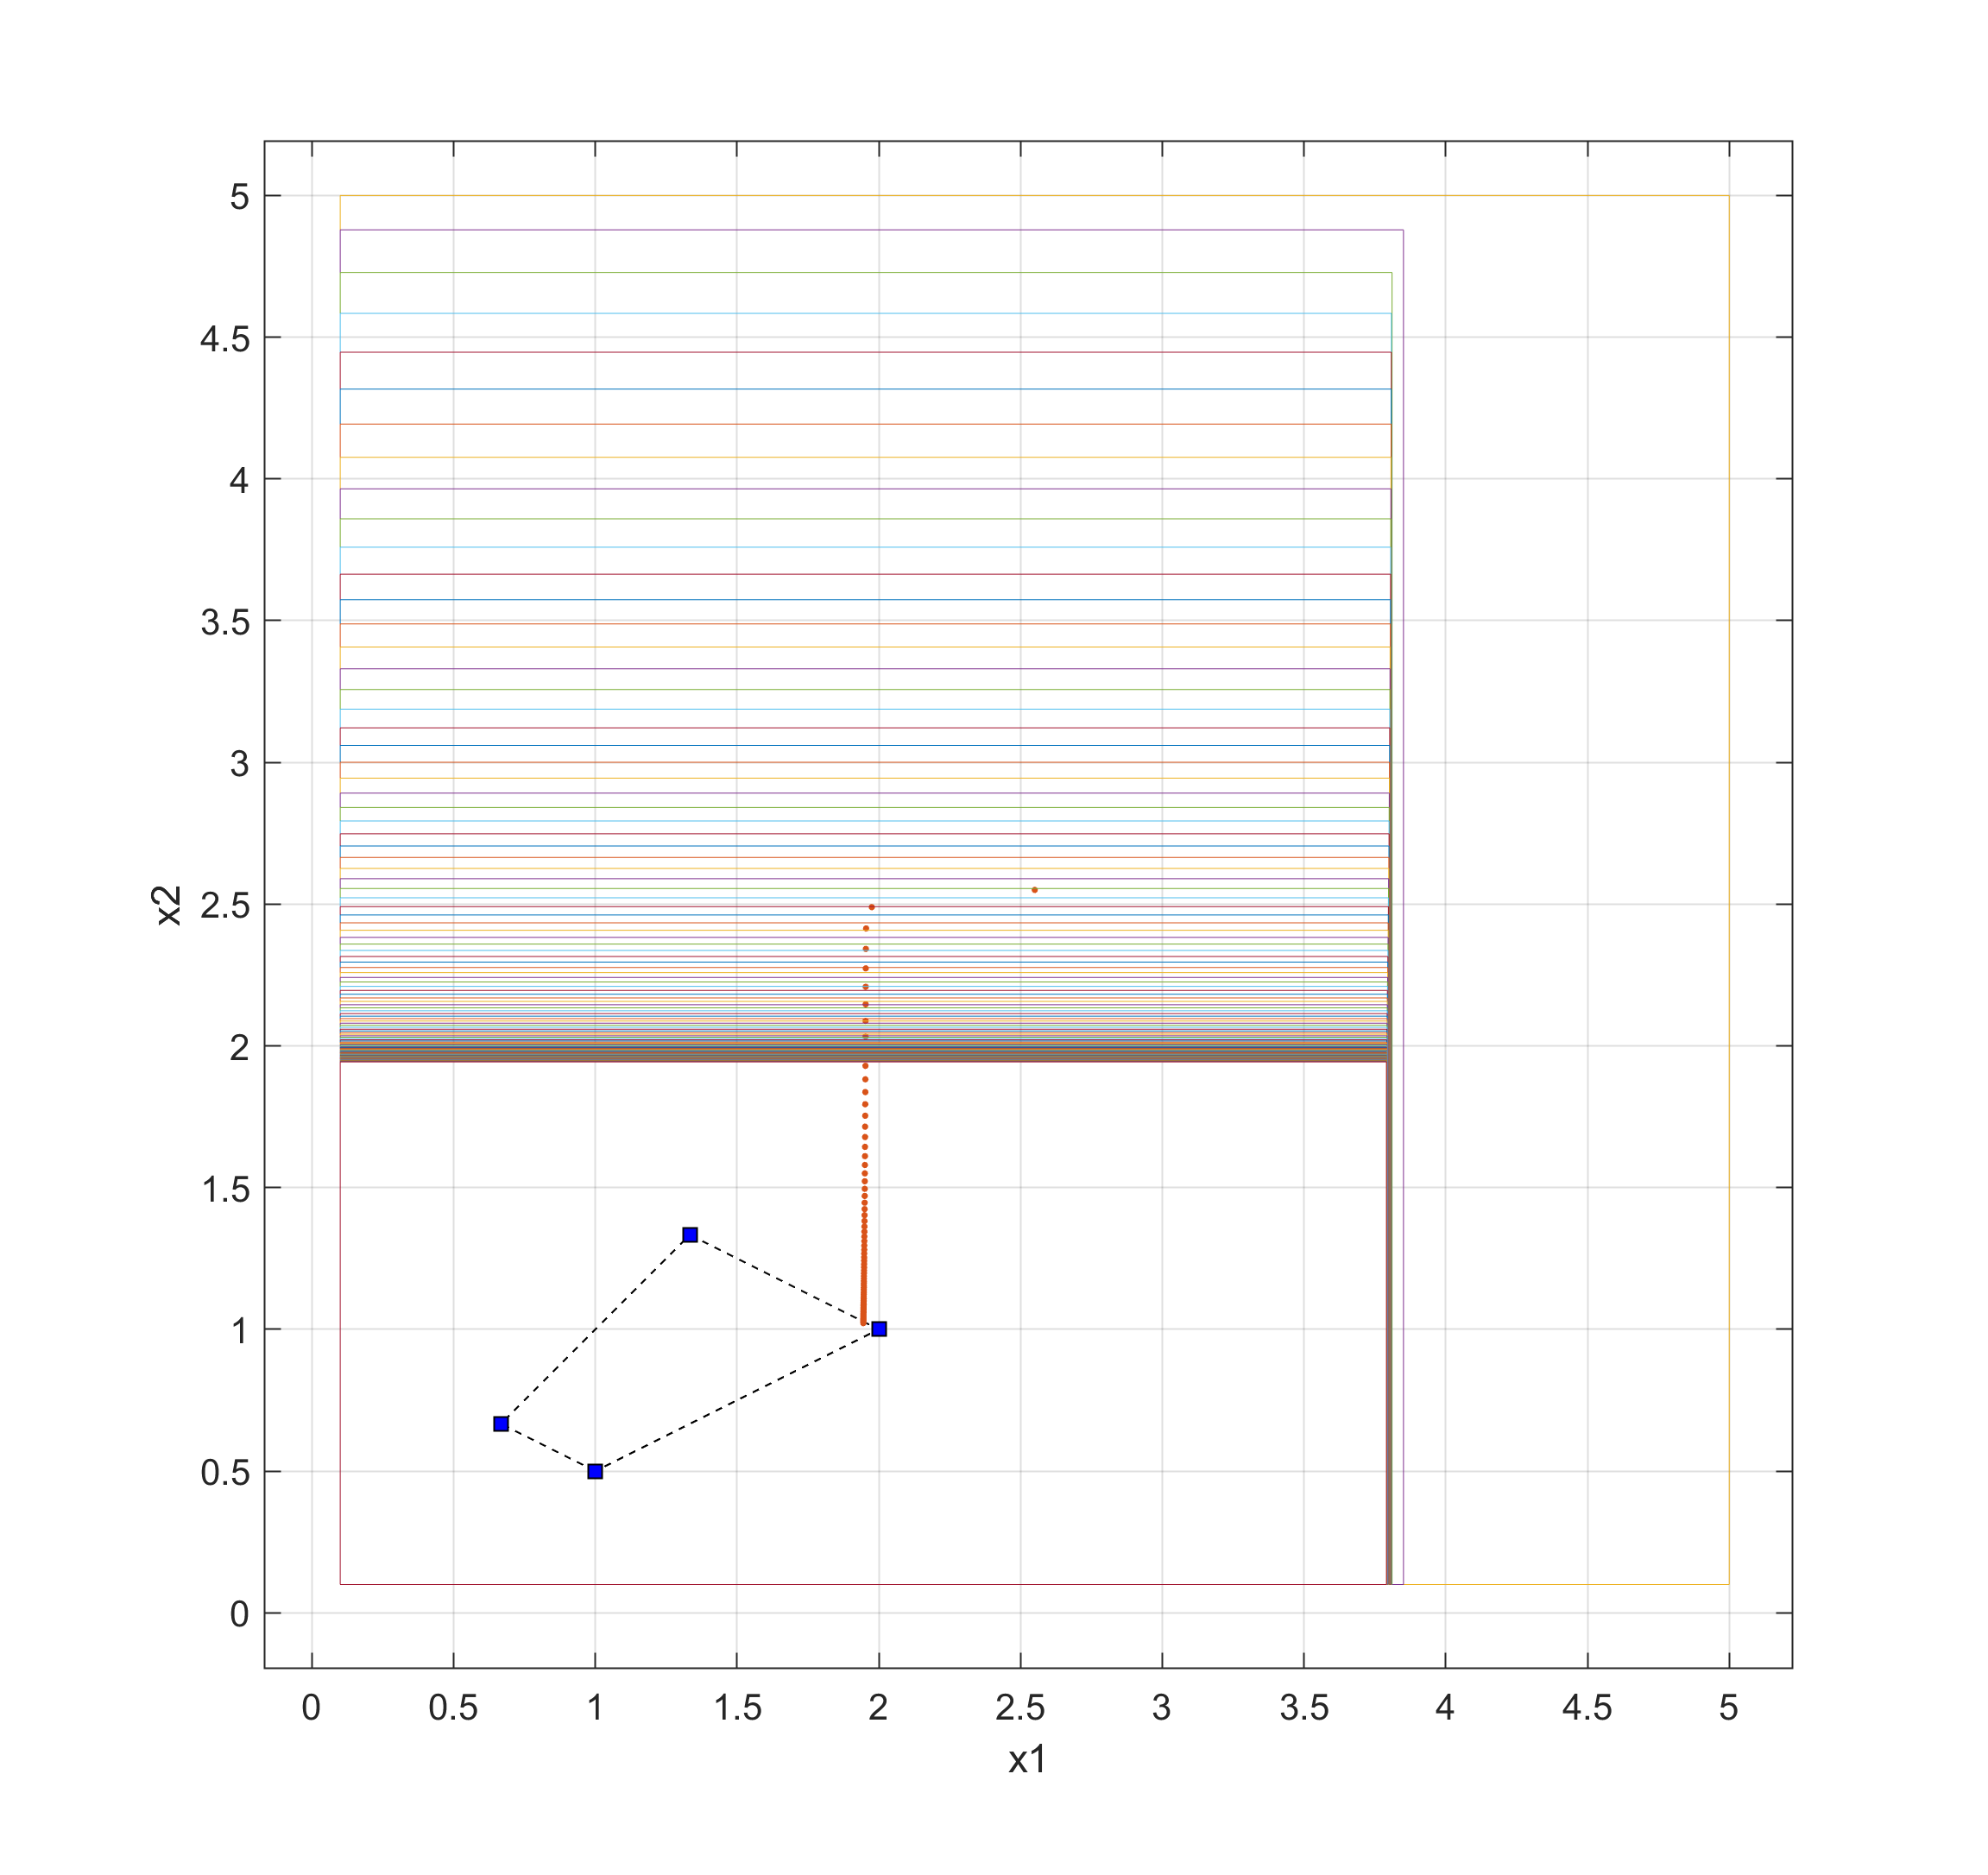
\includegraphics[width=15cm]{img/unlin_mar.png}
    \caption{Иллюстрация работы метода Кравчика для нелинейной системы}
    \label{fig:nelin_krav}
\end{figure}
\begin{figure}[H]
    \centering
    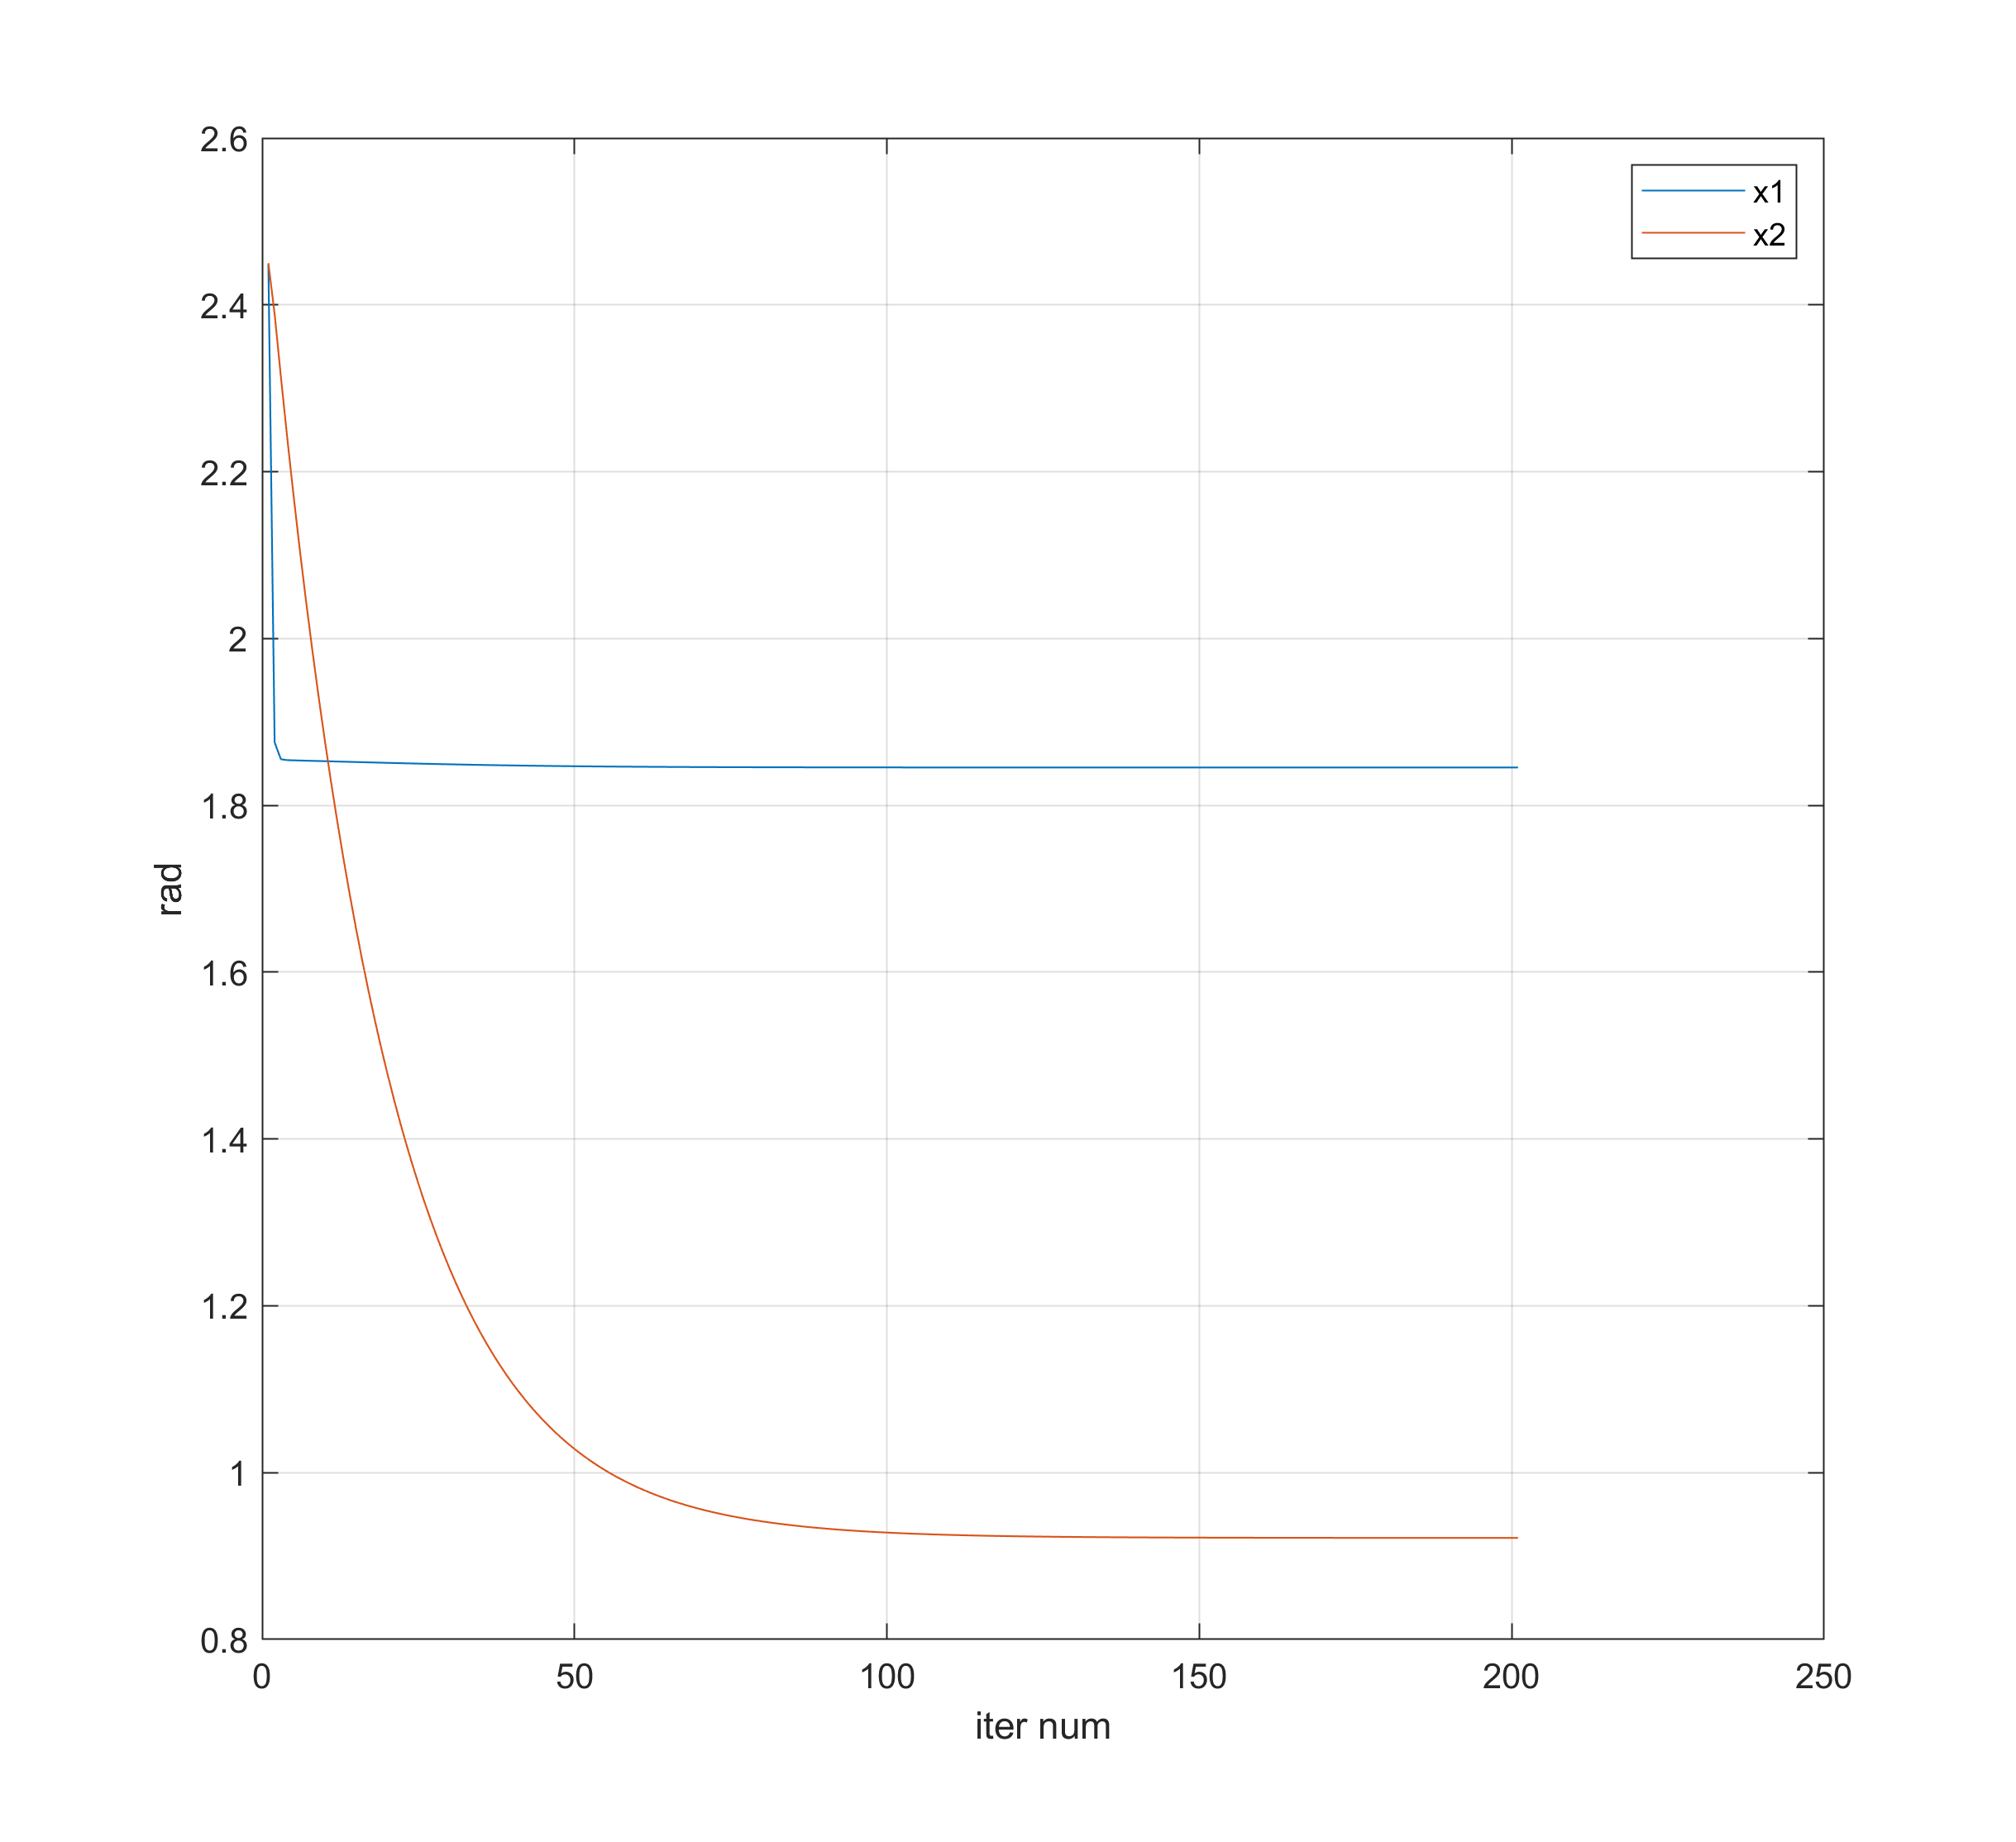
\includegraphics[width=13cm]{img/unlin_rad.png}
    \caption{График радиусов брусов для нелинейной системы}
    \label{fig:nelin_rad}
\end{figure}
\begin{figure}[H]
    \centering
    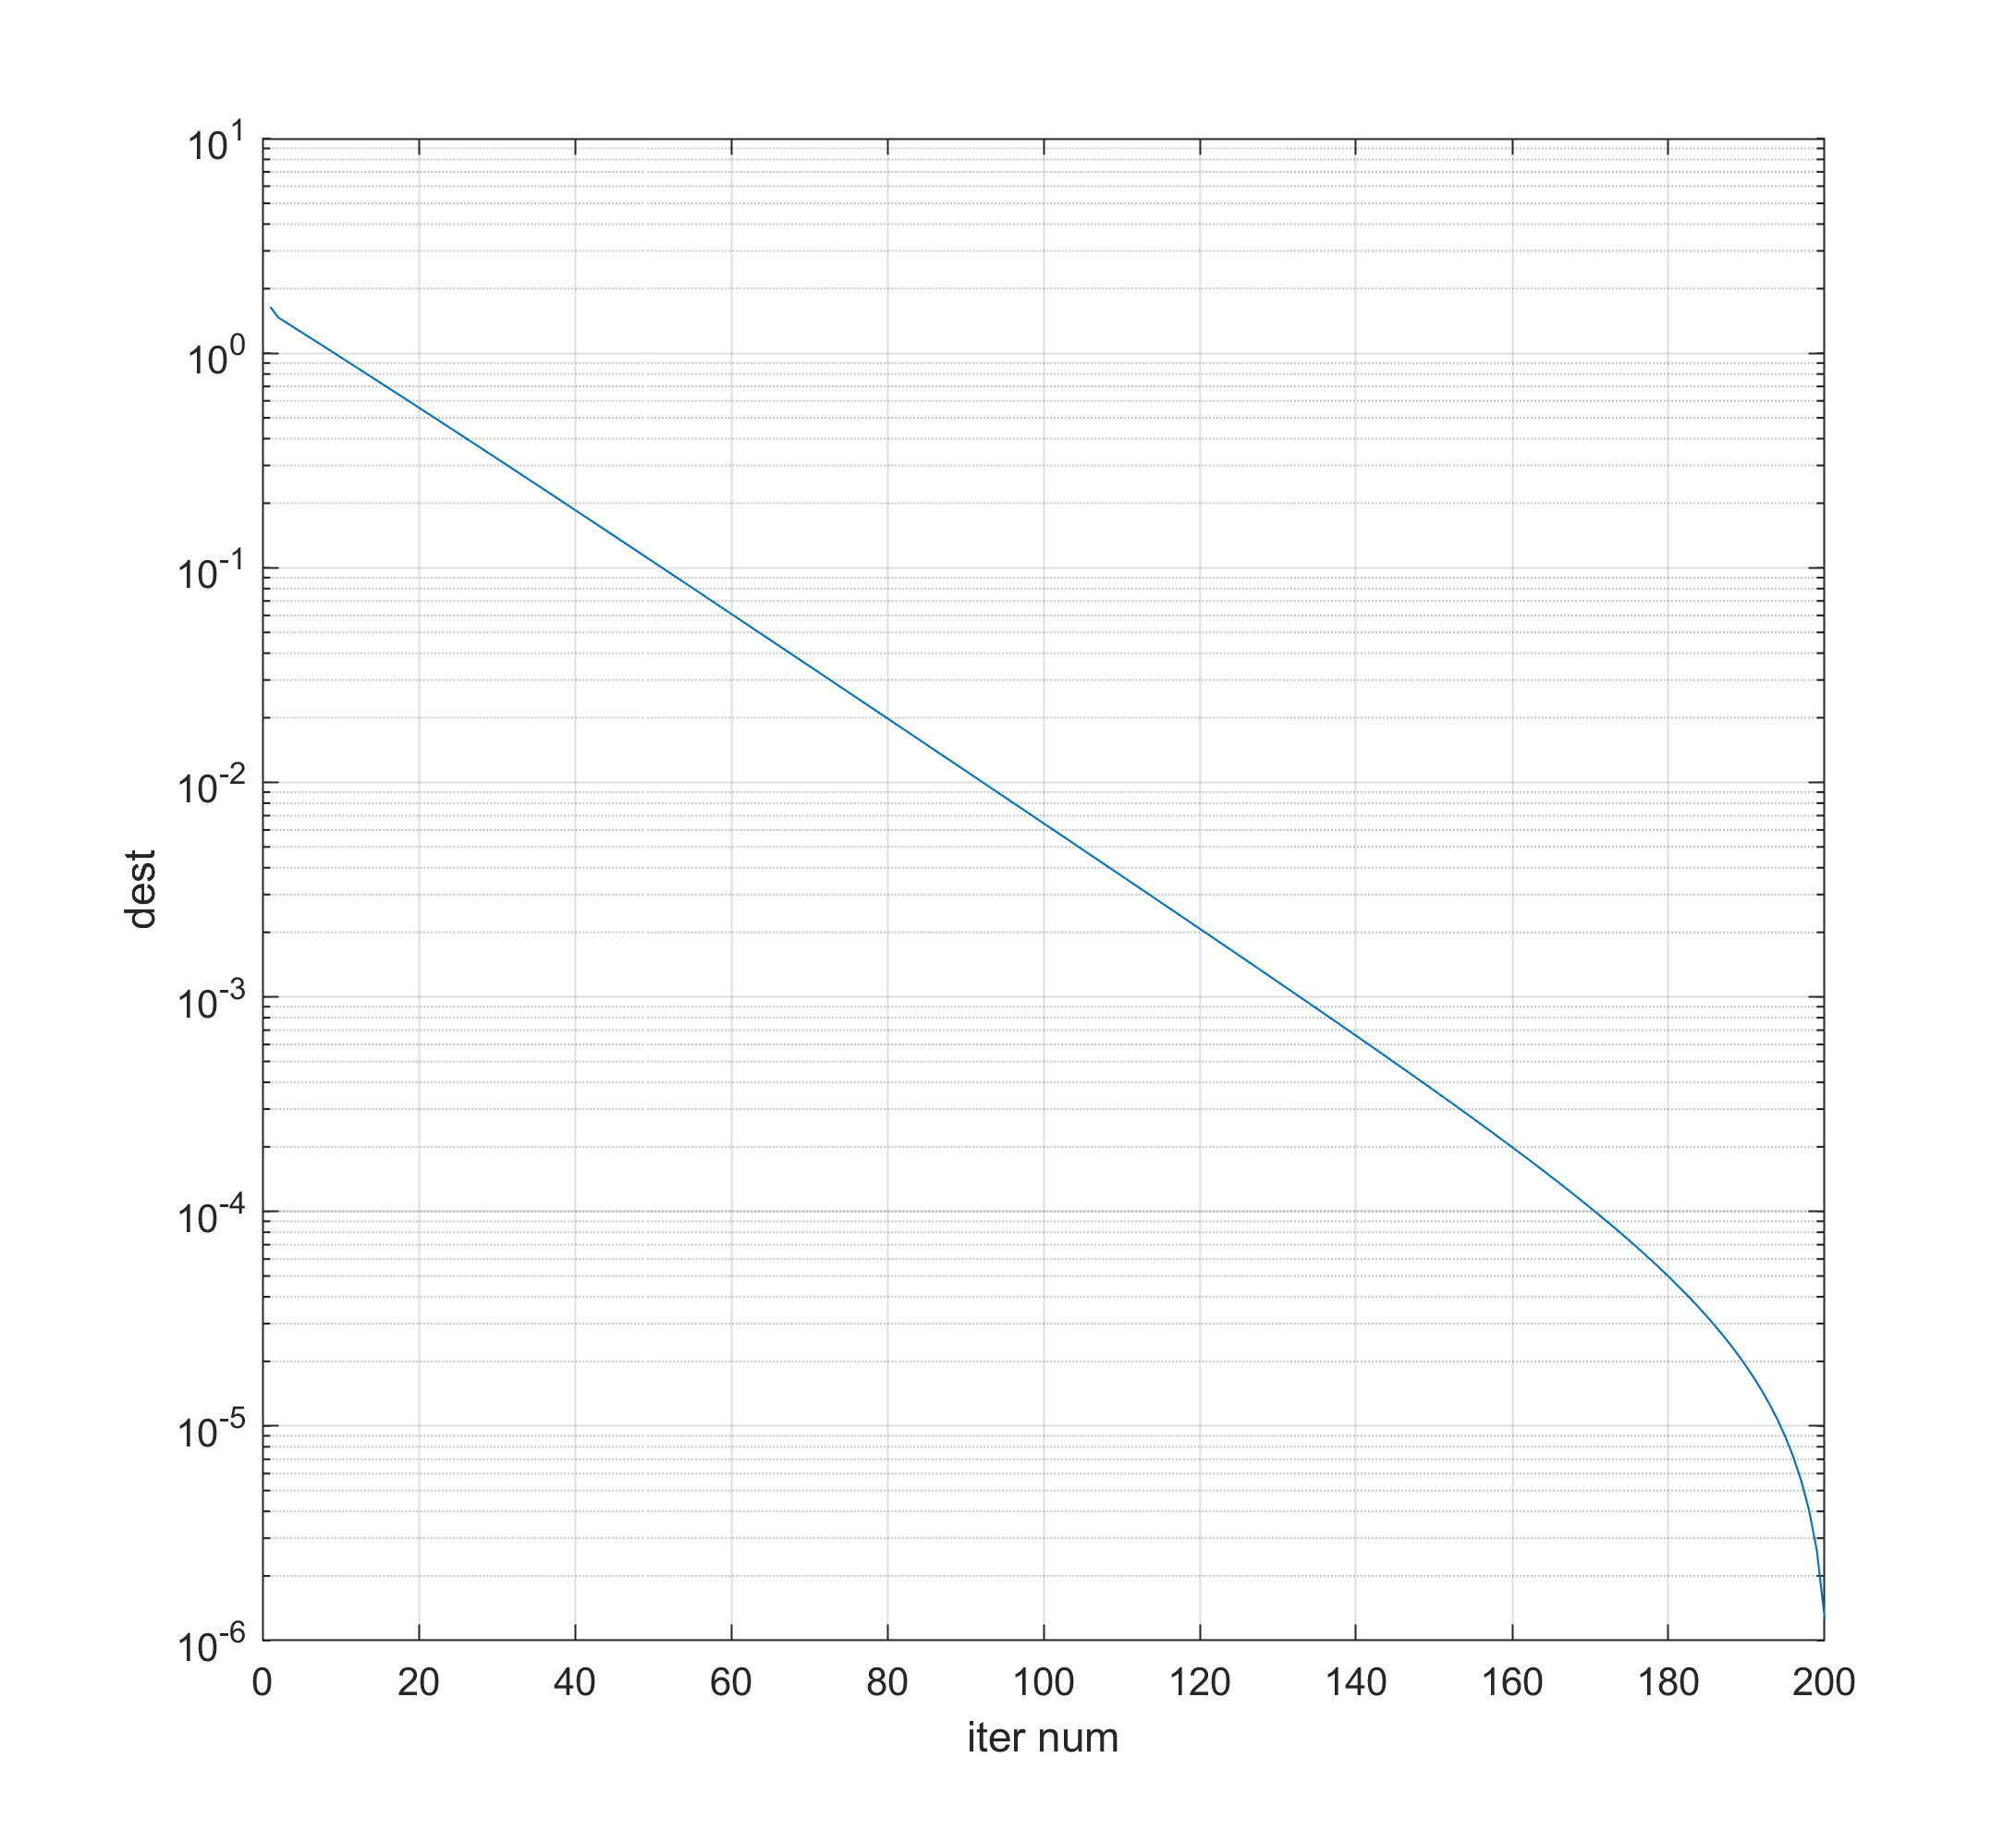
\includegraphics[width=13cm]{img/unlin_dest.png}
    \caption{График сходимости брусов для нелинейной системы}
    \label{fig:nelin_dest}
\end{figure}
\section{Обсуждение}
\begin{enumerate}
    \item Метод Кравчика для ИСЛАУ показал очень быструю сходимость: из грубой начальной оценки метод пришел к брусу, мало отличающемуся от последнего в построенной последовательности, за 4 итерации, если делать вывод на основании графика \ref{fig:islau_rad} радиусов, и за 2 итерации, если делать вывод на основании графика \ref{fig:islau_dest} расстояния между центрами брусов.
    \item Из графика \ref{fig:islau_krav} видно, что на последних итерациях уточняется лишь та грань бруса, по которой и так получено очень точное приближение. Можно сделать вывод, что процесс не сойдется к интервальной оболочке множества $\Xi_{\mathrm{uni}}$.
    \item При решении задачи (\ref{nelin}) была использована начальная оценка так, чтобы брус $\mbf{X}^0$ лежал в первом ортанте, иначе в якобиане появляется операция деления на интервал, содержащий 0. Сходимость более медленная, чем в предыдущем случае.
    \item По графикам \ref{fig:nelin_krav} и \ref{fig:nelin_rad} видно, что вновь в основном происходит уточнение лишь одной грани бруса.
    \item Исходя из графика \ref{fig:nelin_dest} можно сделать вывод, что в отличие от задачи \ref{lin}, в задаче \ref{nelin} движение центра брусов не прекращается даже спустя число итераций, на порядок превосходящее число итераций, на котором остановился предыдущий метод. Тем не менее, сходимость замедляется по мере построений.
    \item Сравнивая графики \ref{fig:islau_krav} и \ref{fig:nelin_krav}, приходим к выводу, что интерпретация задачи как ИСЛАУ дала намного более точное решение. В первом случае получили брус, отличающийся от интервальной оболочки $\Xi_{\mathrm{uni}}$ на величину порядка 0.1 по каждой грани (на одной из граней получено точное значение). В случае рассмотрения задачи как системы нелинейных уравнений получили уточнение лишь по двум граням, погрешность порядка единицы.
\end{enumerate}
\section*{Исходный код}
С исходным кодом программы и отчета можно ознакомиться в репозитории \url{https://github.com/Stasychbr/IntervalArith}.
\end{document}
